\documentclass[]{article}
\usepackage[russian, spanish.mexico]{babel}
\usepackage[T1]{fontenc}
\usepackage[utf8]{inputenc}
%\usepackage{lmodern}
\usepackage[a4paper]{geometry}

%DIAGRAMAS
\usepackage{smartdiagram}
\usesmartdiagramlibrary{additions}
%ARBOLES
%\usetikzlibrary{trees}

%Plotting

\usepackage{pgfplots}
\pgfplotsset{width=10cm,compat=1.9} 
%\usepgfplotslibrary{external}
%\tikzexternalize 

%Graficos e imagenes
\usepackage{graphicx}
%\graphicspath{ Imagenes/ }
\usetikzlibrary{arrows}

\usepackage{natbib}
%\usepackage{cite}

\usepackage{subcaption}

%columnas itemize
\usepackage{multicol}

%Grafico de barras
%\usepackage{pgfplots}
%Arrreglos
\usepackage{array}

\usepackage{tikz}
\usepackage[american voltages, american currents,siunitx]{circuitikz}

\title{Reactores (Boiling Water Reactor) BWR}
\author{Pablo Vivar Colina}
%Comentar para obtener fecha de HOYs
%\date{Octubre 2019}


\begin{document}
	
%%\usepackage[top=2cm,bottom=2cm,left=1cm,right=1cm]{geometry}


\begin{titlepage}
     \begin{center}
	
\includegraphics[width=0.09\textwidth]{UNAM}\Large Universidad Nacional Autónoma de México
        	
\includegraphics[width=0.09\textwidth]{FI}\\[1cm]
        \Large Facultad de Ingeniería\\[1cm]
       % \Large División de Ciencias Básicas\\[1cm]
         \Large Laboratorio de Fundamentos de Control(6655)\\[1cm]
         %la clave antes era:4314
         \footnotesize Profesor: Salcedo Ubilla María Leonor Ing.\\[1cm]
        \footnotesize Semestre 2019-1\\[1cm]
        
       

        \Large Práctica No. 1\\[1cm]
        
           

\Large Introdcción MATLAB
        
         %Texto a la derecha
          \begin{flushright}
\footnotesize  Grupo 2\\[0.5cm]
\footnotesize Brigada: 4\\[0.5cm]
\footnotesize Rodrigo Adrián Martínez López\\[0.5cm]
\footnotesize Vivar Colina Pablo\\[0.5cm]
 \end{flushright}
    %Texto a la izquierda
          \begin{flushleft}
        \footnotesize Ciudad Universitaria Agosto de 2018.\\
          \end{flushleft}
         
          
        %\vfill
        %\today
   \end{center}
\end{titlepage}
 %agregar portada

\maketitle

\tableofcontents  % Write out the Table of Contents



\section{Ventajas BWR}

Desde que el agua es utilizada en la generación de electricidad en este tipo de reactpores, los componentes involucrados como los recalentadores, turbinas y demás deben ser de reforzados, la presión de un BWR es de 7 [MPa] que es la mitad de la presión utilizada en un PWR.\citep{Lamarsh2001}\\

El BWR es un reactor de agua ligera.\\

Junto con el PWR son las tecnologías más utilizadas a lo largo del mundo.\\

Se consideran peligrosos porque se tenía la creencia en los años 50 que las burbujas de vapor le causaban gran inestabilidad.\\

Una de las ventajas de los BWR es que puede ir el vapor directamente a las turbinas a diferencia de un generador PWR por lo que se dice que este tipo de reactores trabaja en ciclo directo.\\[1cm]

Mejoras implementadas de BWR a ABWR:\\

\begin{multicols}{2}
\begin{itemize}
	\item RIPS
	\item Barras de controol
	\item contención primaria
	\item El cuarto de control
	\item fibra optica (mayor velocidad en comunicaciones)
\end{itemize}
\end{multicols}

Mejoras implementadas del ABWR al ESBWR:\\

\begin{multicols}{2}
\begin{itemize}
	\item 1 Sistemas Pasivos de seguridad
	\item Eliminación de los RIPS
	\item Menor Equipo (menor costo y tiempo de mantienimiento)
	\item Contención mejorada
	\item Chimenea ente el núcleo del reactor y separadores de humedad
\end{itemize}
\end{multicols}

Ciclo Rankine (buscar ciclo termodinámico)\\

Los precalentadores de un  BWR tiene que subir la presión a mas de 7.2 [MPa]\\

Para el BWR y el ABWR se controlan con las barras de control y 
con las bombas de recirculacion\\

%Para El ESBWR se controlan con las barras de control y 
%con la temperatura de Agua de Alimentacion\\

%Para el ESWR se tiene un mayor tamaño entre la envolvente y las paredes de la vasija\\

%DBA Design Based Design (Proponer caso catastrofico)\\

%BMAC: parte del ESBWR Estructura que evite que el núcleo se funda\\



%\listoffigures  % Write out the List of Figures

%Resumen de los reactores nucleares tecnología tipo BWR:

\section{BWR-6 General Electric}

\subsection{Diseño}

El Reactor de Agua en Ebullición  es un sistema de generación de vapor de ciclo directo, el combustible  consiste de pastillas cerámicas compuestas dióxido de uranio con un enriquecimiento entre el 3 y 4$\%$.\\

El agua hierve por las fisiones en el núcleo, el vapor húmedo generado pasa a través de los secadores de vapor,  saliendo con una calidad de 0.30 $\%$ de humedad y una presión entre 970 a 1000 [psi] y se envía directamente a la turbina.\\

Después de haber pasado por la turbina, el vapor es condensado y bombeado a través de los desmineralizadores, precalentadores de agua de alimentación y por último, regresado a la vasija del reactor para así completar el ciclo.\\

La vasija del reactor, los internos y los mecanismos de accionamiento de las barras de control. El núcleo del reactor, los separadores de vapor, los secadores de vapor, el soporte y posicionamiento del núcleo. \\



Se tienen tres direcciones de flujo en la vasija:\\


\begin{itemize}
	 
	\item El agua entra a la vasija por medio de la penetración de entrada de agua de alimentación
	
\item Del ánulo, vía la penetración de salida del agua de recirculación  
	
\item El excedente entra en la succión de las bombas jet.
	
\end{itemize}

Los tres flujos se juntan en los difusores de las bombas jet y se descargan al parte inferior del núcleo.\\

El agua fluye hacia la parte superior donde una porción del líquido es convertida en vapor, el líquido separado del vapor regresa ánulo, para reciclarse, y el vapor es enviado a la turbina. El vapor saturado deja la vasija  por medio de cuatro líneas de vapor principal, dos válvulas de aislamiento y dos grupos de válvulas de seguridad-alivio.\\

El vapor desfogado por cualquier grupo de válvulas de alivio de seguridad es descargado en la alberca de supresión.\\

El sistema principal de vapor suministra el vapor para el turbogenerador, las turbinas de las bombas de alimentación, los recalentadores de vapor y para componentes auxiliares.\\

El vapor  llega al domo pasando por los separadores y secadores haciendo que el fluido con mayor densidad se desplace radialmente y se separe del vapor.\\

%Características de diseño de cada reactor.
\begin{figure}[h!]
	\centering
	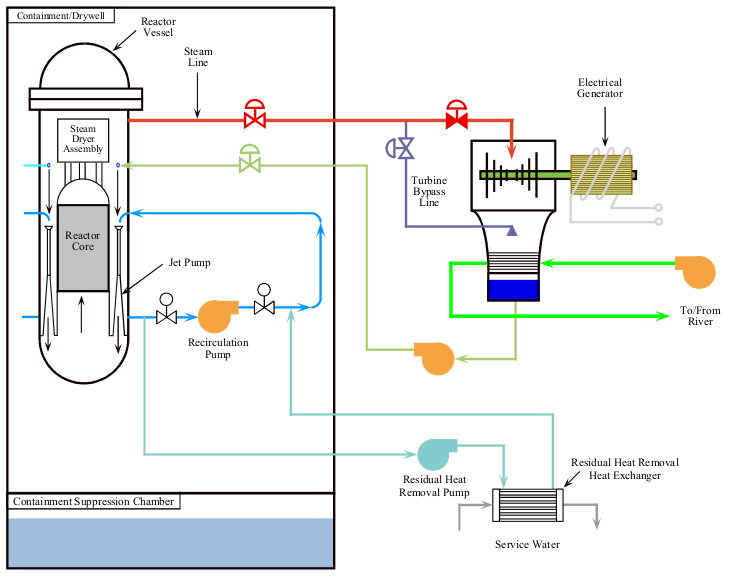
\includegraphics[width=0.8\textwidth]{ReactorBWR.png}
	\caption{Componentes de la planta BWR}
	\label{fig:ReactorBWR}
\end{figure}


%\subsection{Combustible}
%Características del combustible.

%\subsection{Accidentes de Base de Diseño}
%Descripción del DBA para cada reactor.
%design basis accidents (DBA)

%De acuerdo con GDC 26, GDC 28 y GDC 29 (Ref. 1), la reactividad
%será controlable de manera que la subcrítica se mantenga en frío
%las condiciones y los límites de diseño de combustible aceptables no se excedan durante
%el funcionamiento normal y las incidencias operativas previstas. 


\subsection{Reactividad}
se utiliza como una medida de la predicción contra el núcleo medido
reactividad durante la operación de potencia. La confirmación continua de los valores
reactividad es necesaria para asegurar que la base de diseño del accidente (DBA)
y los análisis de seguridad de transitorios siguen siendo válidos. Una gran anomalía de reactividad
podría ser el resultado de cambios imprevistos en la reactividad del combustible, la varilla de control
o en condiciones que no sean consistentes con las asumidas en la Ley de la
predicciones de la reactividad del núcleo, y podría resultar potencialmente en una pérdida de SDM
o violación de los límites de diseño de combustible aceptable. Comparación de las predicciones con los resultados
la reactividad medida del núcleo valida los métodos nucleares utilizados en la seguridad
y apoya las demostraciones de MDF (LCO 3.1.1.),
"(SHUTDOWN MARGIN (SDM)") para asegurar que el reactor pueda ser traído
de forma segura a condiciones frías y subcríticas.\\\citep{Regulation}

%%DBA 2

La comparación entre la reactividad inicial medida y la prevista del núcleo
proporciona una normalización para los modelos de cálculo utilizados para predecir el núcleo
reactividad. Si el k eff medido y predicho para condiciones centrales idénticas
en BOC no concuerdan razonablemente, entonces las suposiciones utilizadas en la recarga
el análisis del diseño del ciclo o los modelos de cálculo utilizados para predecir k eff pueden
no ser preciso. Si existe un acuerdo razonable entre el valor medido y el
la reactividad prevista del núcleo existe en el COB, entonces la predicción puede ser
normalizado al valor medido. A partir de entonces, cualquier desviación significativa
en el k eff medido a partir del k eff previsto que se desarrolla durante la combustión
el agotamiento puede ser una indicación de que las suposiciones del DBA y la
los análisis transitorios ya no son válidos, o que un cambio inesperado de
de las condiciones básicas.\citep{Regulation}\\

%DBA2

Si un subsistema del sistema SLC no puede funcionar por razones que no sean
Condición A: el subsistema inutilizable deberá restablecerse a "OPERABLE".
en un plazo de 7 días. En esta condición, el resto de la unidad OPERABLE
es adecuado para realizar la función de apagado. Sin embargo, el
la fiabilidad general se reduce debido a que una sola falla en el resto del sistema
El subsistema OPERABLE podría resultar en una reducción de la parada del sistema SLC.
capacidad. El Tiempo de Terminación de 7 días está basado en la disponibilidad de un
Subsistema OPERABLE capaz de realizar el sistema SLC previsto
y la baja probabilidad de un accidente con base en el diseño (DBA) o
transitorios severos que ocurren simultáneamente con la falla de la varilla de control
Sistema de accionamiento para el cierre de la planta.\citep{Regulation}\\




\subsection{Situación Actual}
%Situación actual de estos reactores.

Son reactores de segunda generación que fueron muy populares en la década de los 80, pero que en la actualidad no hay proyecciones para nuevas construcciones de reactores de este tipo ya que los fabricantes de vasijas se han orientado a la elaboración de reactores de tercera generación. Aún así existen en el mundo reactores con este tipo de tecnología aún en operación como es el de laguna verde.\\

%Diferencias entre estos Reactores.

\section{ABWR General Electric, Hitachi}

\begin{figure}[h!]
	\centering
	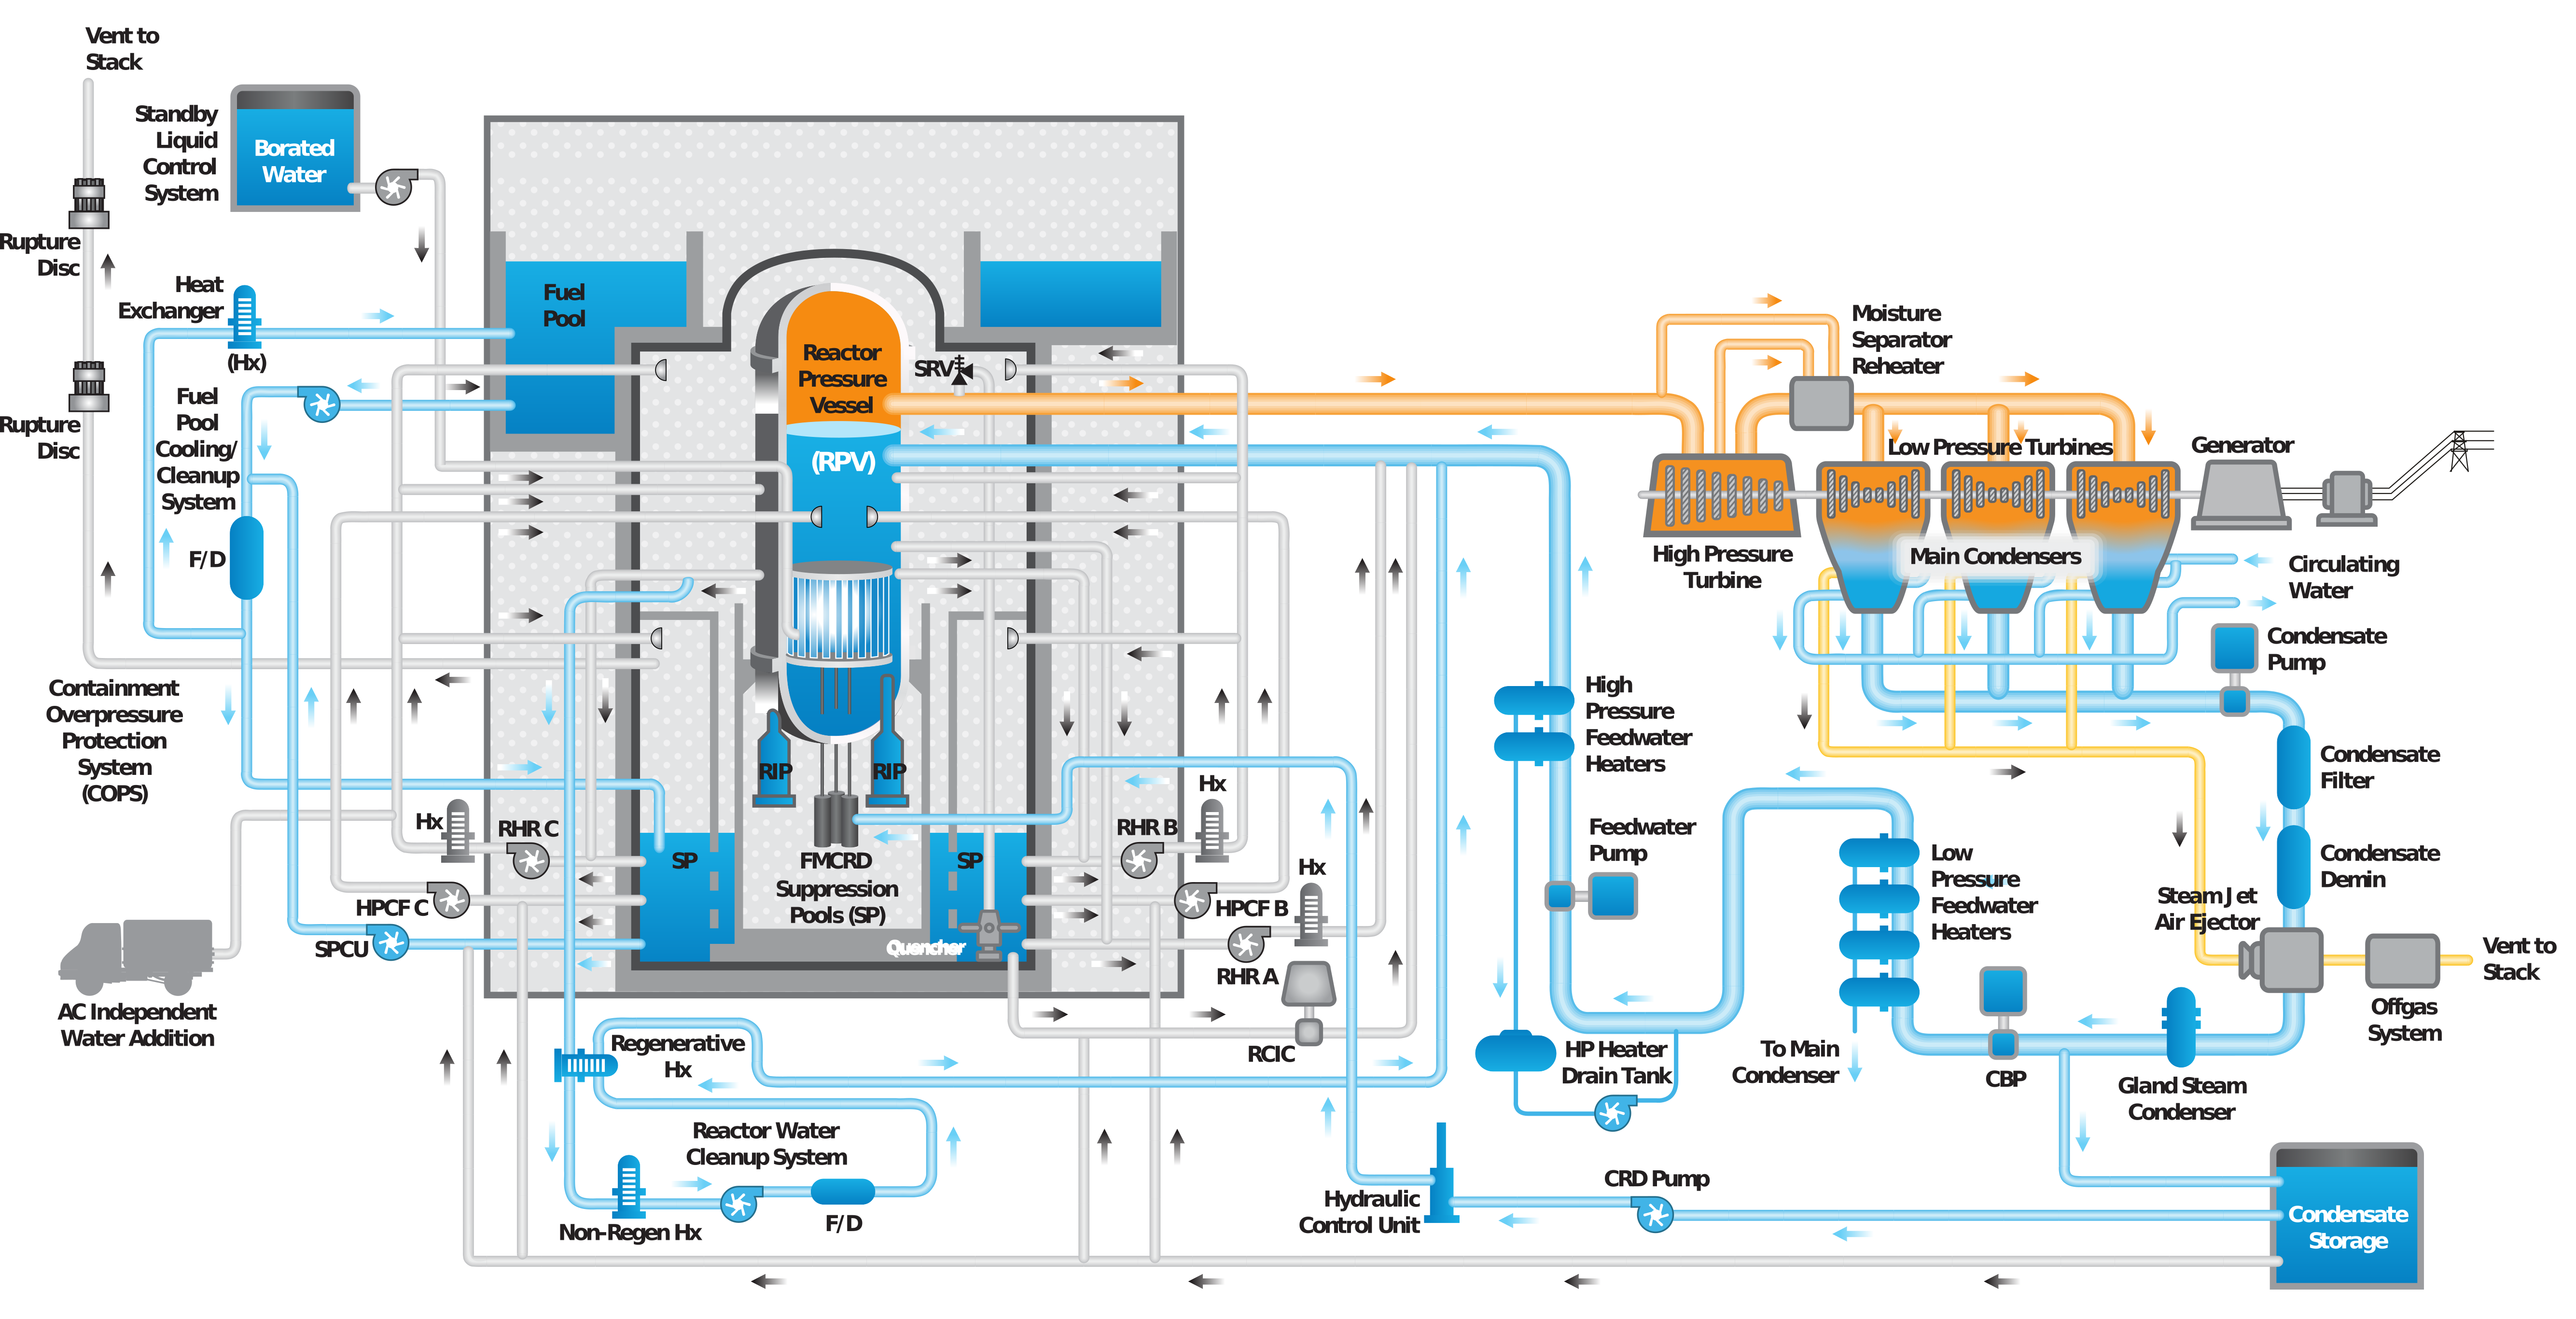
\includegraphics[width=0.99\textwidth]{diagramaABWR.png}
	\caption{Componentes de la planta ABWR \citep{Hitachi2007}}
	\label{fig:ReactorABWR}
\end{figure}


\subsection{Diseño}
%Características de diseño de cada reactor.

\begin{table}[h!]
	\begin{tabular}{||c|p{5cm}|p{5cm}||}
		\hline
		\textbf{Característica}       & \textbf{ABWR}                                   & \textbf{BWR/6}                                          \\ \hline\hline
		Recirculación                 & Bombas integradas a vasija del reactor          & Dos circuitos de recirculacióncon bombas jet integradas \\ \hline
		Barras de control             & Movimiento fino                                 & Aseguramiento por pistones                               \\ \hline
		Vasija de Reactor             & Anillos forjados                                & Placas                                                  \\ \hline
		Control e Instrumentación     & Digital, multiplexado, fibra óptica, multicanal & Analógico de un canal                                   \\ \hline
		Mitigación de Accidente grave & Inerte, ventilación de contaminante             & No especificada                                         \\ \hline
		Limpieza de Reactor de agua   & 2 $\%$ bombas en pierna fría            & 1 $\%$ en pierna caliente                       \\ \hline
	\end{tabular}
\caption{Tabla comparativa ABWR y BWR/6}
\label{cuad:CompABWRyBWR6}
\end{table}

%\subsection{Combustible}
%Características del combustible.

%\subsection{Accidentes de Base de Diseño}
%Descripción del DBA para cada reactor.
%design basis accidents (DBA)

%\subsection{Situación Actual}
%Situación actual de estos reactores.

%Diferencias entre estos Reactores.


\section{ESBWR General Electric, Hitachi, Toshiba}

\subsection{Introducción}

Desde su participación en la construcción del BWR en la Unidad 1 de la Central Eléctrica de Tsuruga (357 MWe) para The Japan Atomic Power Compañía en 1970, Hitachi ha completado con éxito la construcción de de más de 20 centrales nucleares.\\

%Durante 1996 y 1997 Hitachi se unió a General Electric Company de los EE.UU. y Toshiba Corporation para completar la construcción de los dos primeros ABWR en las Unidades 6 y 7 del
%Central nuclear Kashiwazaki-Kariwa de la Tokyo Electric Power. Desde entonces, Hitachi ha emprendido una amplia gama de actividades nucleares. De desarrollo de reactores para satisfacer las necesidades de los clientes sobre la base de su
%experiencia en el diseño y construcción de todos los ABWRs hasta la fecha,
%tanto dentro como fuera de Japón, e incluyendo las plantas en la fase de planificación.
%Ahora, por primera vez en unos veinte años, un proyecto nacional ha sido
%iniciado en Japón para desarrollar un nuevo reactor de agua ligera. Además de
%Como protagonista de este proyecto

 Hitachi también está trabajando con General Electric
en los EE.UU. sobre el diseño y las pruebas de confirmación como parte de la ESBWR
proyecto de desarrollo.\citep{Matsuura2009}\\

\subsection{Diseño}
%Características de diseño de cada reactor.
%DESARROLLO DE ESBWR
%Características
El ESBWR (reactor de agua económico y simplificado) es un reactor de circulación natural para alta presión.\\

plantas de producción (1.550 MWe) desarrolladas sobre la base de las tecnologías de GE.
experiencia con el ABWR y con el SBWR
(reactor de agua hirviendo simplificado) en el que Hitachi
también jugó un papel en el desarrollo. El diseño del reactor.\citep{Matsuura2009}\\

\begin{figure}[h!]
	\centering
	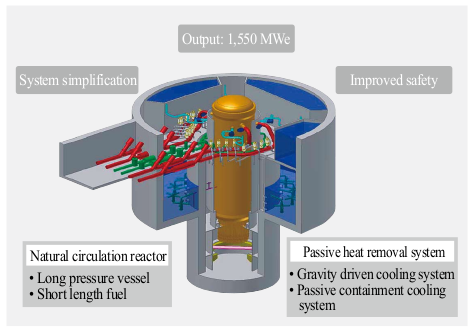
\includegraphics[width=0.8\textwidth]{ReactorESBWR.png}
	\caption{Componentes de la planta ESBWR}
	\label{fig:ReactorESBWR}
\end{figure}


Persigue el concepto de un simple reactor nuclear algo que es una característica de los BWRs. Este reactor simplificado de alto rendimiento utiliza una tecnología natural de
sistema de reactor de circulación que elimina la necesidad de
para una bomba de recirculación de refrigerante del reactor y seguridad
equipo que utiliza sistemas pasivos como un
condensador de emergencia, refrigeración por gravedad del reactor,
y la refrigeración pasiva de los recipientes de contención para reducir
la cantidad de equipos mediante la eliminación de los activos
componentes como las bombas, a la vez que se reducen
costes de funcionamiento y mantenimiento (véase la Fig. \ref{fig:ReactorESBWR}).\\


%Empresa Común que utiliza sinergias con GE
%Junto con el ABWWR, 
El ESBWR es un valioso tipo de reactor capaz de hacer frente a la repentina afluencia de energía nuclear la construcción de centrales eléctricas que ha surgido en los EE.UU.
GE está asumiendo un papel de liderazgo en la obtención de normas en los EE.UU. y solicitó la aprobación de US DC (diseño) en agosto de 2005. Además de asistir en estos asuntos regulatorios a través de análisis y otras contribuciones, Hitachi está utilizando sus capacidades de diseño y fabricación de equipos para apoyar el diseño detallado de los equipos con nuevos elementos de diseño como los componentes internos del reactor, el control
y recipiente de contención.\\

La capacidad de utilizar la circulación natural es la clave de la ESBWR y logra el núcleo requerido. De la chimenea en la parte superior del edificio. y la obtención de su fuerza motriz a partir de la diferencia en la densidad del refrigerante. La chimenea es una gran pieza de en el reactor con una altura de aproximadamente 7 m y de unos 6 m de diámetro. La chimenea está situada en la parte superior del núcleo y actúa como un túnel para el flujo bifásico (flujo mixto de agua y vapor) que se genera desde el interior del núcleo. A estructura de chimenea dividida con una malla cuadrada. Se utiliza para forzar este flujo de dos fases fluya libremente sin convertirse en estacionario. La chimenea es la más característica y
importante componente de la ESBWR de Hitachi.\citep{Matsuura2009}\\
%De esta manera, Hitachi prestará su "fabricación", "ingeniería
%capacidad" y "capacidad de investigación y desarrollo".
%las fortalezas de la ESBWR para hacer preparativos exhaustivos
%para la construcción de instalaciones reales en combinación con
%GE (véase la Fig. 9).\citep{Matsuura2009}\\\\

%\subsection{Operación}

Para el EBSWR se tiene un mayor tamaño entre la envolvente y las paredes de la vasija. Las barras de control son el punto de regulación de fisiones dentro del reactor, además de ello otro punto de regulación es la temperatura de Agua de Alimentación la cual cambiando su densidad a una menor puede causar menos fisiones.\\

%\subsection{Combustible}
%Características del combustible.

%\subsection{Accidentes de Base de Diseño}
%Descripción del DBA para cada reactor.
%design basis accidents (DBA)

\subsection{Situación Actual}

Este tipo de reactores sigue en etapa experimental y de pruebas por parte de las compañías antes mencionadas, y se pretende comenzar a construir para el año 2020 alguna planta nuclear con reactores de este tipo en E.E.U.U. o en Japón. situación que presenta un reto debido al reciente accidente nuclear en Fukishima y la nueva política de generación energética en Japón.\\

%DBA Design Based Design (Proponer caso catastrofico)\\
%BMAC: parte del ESBWR Estructura que evite que el núcleo se funda\\
%Situación actual de estos reactores.
%Diferencias entre estos Reactores.



%El resumen para cada tipo de reactor, tomando como idea el poder compararlos con el
%reactor BWR/6 (Igual al de la CNLV), para entender los cambios y mejoras realizados
%en este tipo de reactores:


\section{Conclusiones}

La construcción de las centrales nucleares está cobrando impulso en todo el mundo, este trabajo cumpló su objetivo porque se logró describir los avances sobre el tipo de tecnología de reactores BWR y sus correspondientes mejoras en loas años y mejora continua para las nuevas versiones.\\

 Es necesario la construcción de las centrales nucleares a nivel internacional como un instrumento eficaz para prevenir el calentamiento global, y el ESBWR puede tomar un papel importante en ese proceso.\\

%es necesario que el Japón mejore su capacidad técnica y técnica.
%(en particular, las competencias técnicas del país.
%en la construcción) que han atraído genuinamente a la
%el interés y las expectativas del mundo en general y
%prepararse para la era venidera de la construcción extensiva
%actuación

\bibliographystyle{plain}
\bibliography{Referencias.bib}

\end{document}
